\documentclass[border=10pt]{standalone}
\usepackage{tikz}
\usepackage{tikz-uml}

\begin{document}

\begin{tikzpicture}

% ============================================================================
% Core Environment Class
% ============================================================================

\umlclass[x=0, y=-6]{Environment}{
  - \_use\_simulation : bool \\
  - \_verbose : bool \\
  - \_robot : Robot \\
  - \_framegrabber : FrameGrabber \\
  - \_workspaces : Workspaces \\
  - \_oralcom : Text2Speech \\
  - \_visual\_cortex : VisualCortex \\
  - \_stop\_event : Event \\
  - \_obj\_position\_memory : Objects \\
  - \_memory\_lock : Lock \\
  - \_is\_at\_observation\_pose : bool \\
  - \_workspace\_was\_lost : bool
}{
  + \_\_init\_\_(el\_api\_key, use\_simulation, robot\_id, verbose) \\
  + cleanup() \\
  + start\_camera\_updates(visualize) : Thread \\
  + update\_camera\_and\_objects(visualize) : Iterator \\
  + clear\_memory() \\
  + remove\_object\_from\_memory(label, coord) \\
  + get\_detected\_objects\_from\_memory() : Objects \\
  + get\_current\_frame() : ndarray \\
  + get\_detected\_objects() : Objects \\
  + get\_workspace(index) : Workspace \\
  + get\_robot\_pose() : PoseObjectPNP \\
  + robot\_move2observation\_pose(workspace\_id) \\
  + add\_object\_name2object\_labels(name) : str \\
  + get\_largest\_free\_space\_with\_center() : Tuple \\
  - \_should\_update\_memory() : bool \\
  - \_should\_clear\_memory() : bool \\
  - \_check\_new\_detections(objects)
}

% ============================================================================
% Camera Classes
% ============================================================================

\umlclass[x=-10, y=8]{FrameGrabber}{
  \{abstract\} \\
  - \_current\_frame : ndarray \\
  - \_environment : Environment \\
  - \_verbose : bool
}{
  + \_\_init\_\_(environment, verbose) \\
  + \{abstract\} get\_current\_frame() : ndarray \\
  + get\_current\_frame\_shape() : Tuple \\
  + get\_current\_frame\_width\_height() : Tuple \\
  + current\_frame() : ndarray \\
  + environment() : Environment \\
  + verbose() : bool
}

\umlclass[x=-19, y=2]{NiryoFrameGrabber}{
  - \_robot : NiryoRobotController \\
  - \_mtx : ndarray \\
  - \_dist : ndarray \\
  - streamer : RedisImageStreamer \\
  - frame\_counter : int
}{
  + \_\_init\_\_(environment, stream\_name, verbose) \\
  + get\_current\_frame() : ndarray \\
  + publish\_workspace\_image(image, ws\_id, pose) \\
  + is\_point\_visible(world\_point, transform) : bool \\
  + camera\_matrix() : ndarray \\
  + camera\_dist\_coeff() : ndarray
}

\umlclass[x=-19, y=8]{WidowXFrameGrabber}{
}{
  + \_\_init\_\_(environment, verbose) \\
  + get\_current\_frame() : ndarray
}

% ============================================================================
% Robot Classes
% ============================================================================

\umlclass[x=14, y=-14]{RobotAPI}{
  \{abstract\}
}{
  + \{abstract\} pick\_place\_object(...) : bool \\
  + \{abstract\} pick\_object(name, coord) : bool \\
  + \{abstract\} place\_object(coord, location) : bool \\
  + \{abstract\} push\_object(name, coord, dir, dist) : bool \\
  + move2observation\_pose(workspace\_id)
}

\umlclass[x=14, y=-7]{Robot}{
  - \_environment : Environment \\
  - \_verbose : bool \\
  - \_robot : RobotController \\
  - \_object\_last\_picked : Object \\
  - \_robot\_in\_motion : bool
}{
  + \_\_init\_\_(environment, use\_sim, robot\_id, verbose) \\
  + pick\_place\_object(name, pick\_c, place\_c, loc) : bool \\
  + pick\_object(name, coordinate) : bool \\
  + place\_object(coordinate, location) : bool \\
  + push\_object(name, coord, direction, distance) : bool \\
  + move2observation\_pose(workspace\_id) \\
  + get\_pose() : PoseObjectPNP \\
  + get\_target\_pose\_from\_rel(...) : PoseObjectPNP \\
  + environment() : Environment \\
  + robot\_in\_motion() : bool \\
  - \_get\_nearest\_object(label, coords) : Object
}

\umlclass[x=14, y=2]{RobotController}{
  \{abstract\} \\
  - \_lock : Lock \\
  - \_verbose : bool \\
  - \_robot : Robot \\
  - \_robot\_ctrl : Object
}{
  + \_\_init\_\_(robot, use\_simulation, verbose) \\
  + \{abstract\} get\_pose() : PoseObjectPNP \\
  + \{abstract\} robot\_pick\_object(obj) : bool \\
  + \{abstract\} robot\_place\_object(pose) : bool \\
  + \{abstract\} robot\_push\_object(pose, dir, dist) : bool \\
  + \{abstract\} get\_target\_pose\_from\_rel(...) : PoseObjectPNP \\
  + \{abstract\} move2observation\_pose(workspace\_id) \\
  + lock() : Lock \\
  + verbose() : bool \\
  - \{abstract\} \_init\_robot(use\_simulation) : bool
}

\umlclass[x=0, y=6]{NiryoRobotController}{
  - \_robot\_ip\_address : str \\
  - \_executor : ThreadPoolExecutor \\
  - \_shutdown\_v : bool
}{
  + \_\_init\_\_(robot, use\_simulation, verbose) \\
  + cleanup() \\
  + get\_pose() : PoseObjectPNP \\
  + get\_camera\_intrinsics() : Tuple \\
  + get\_img\_compressed() : ndarray \\
  + robot\_pick\_object(obj) : bool \\
  + robot\_place\_object(pose) : bool \\
  + robot\_push\_object(pose, dir, dist) : bool \\
  + get\_target\_pose\_from\_rel(...) : PoseObjectPNP \\
  + move2observation\_pose(workspace\_id) \\
  + reset\_connection() \\
  - \_create\_robot() \\
  - \_init\_robot(use\_simulation) : bool \\
  - \_shutdown() \\
  - \_move\_pose(pose) \\
  - \_shift\_pose(axis, distance)
}

\umlclass[x=11, y=9]{WidowXRobotController}{
}{
  + \_\_init\_\_(robot, use\_simulation, verbose) \\
  + get\_pose() : PoseObjectPNP \\
  + robot\_pick\_object(obj) : bool \\
  + robot\_place\_object(pose) : bool \\
  + robot\_push\_object(pose, dir, dist) : bool \\
  + get\_target\_pose\_from\_rel(...) : PoseObjectPNP \\
  + move2observation\_pose(workspace\_id) \\
  - \_init\_robot(use\_simulation) : bool
}

% ============================================================================
% External Package Classes (Simplified)
% ============================================================================

\umlclass[x=-12, y=-9]{VisualCortex}{
  \{external: vision\_detect\_segment\}
}{
  + detect\_objects\_from\_redis() \\
  + get\_detected\_objects() : List[Dict] \\
  + get\_annotated\_image() : ndarray \\
  + add\_object\_name2object\_labels(name) \\
  + get\_object\_labels() : List[List[str]]
}

\umlclass[x=-12, y=-14]{Text2Speech}{
  \{external: text2speech\}
}{
  + call\_text2speech\_async(text) : Thread
}

\umlclass[x=-19, y=-4]{RedisImageStreamer}{
  \{external: redis\_robot\_comm\}
}{
  + publish\_image(image, metadata, ...) : str
}

% ============================================================================
% Relationships
% ============================================================================

% Inheritance
\umlinherit{NiryoFrameGrabber}{FrameGrabber}
\umlinherit{WidowXFrameGrabber}{FrameGrabber}
\umlinherit{Robot}{RobotAPI}
\umlinherit{NiryoRobotController}{RobotController}
\umlinherit{WidowXRobotController}{RobotController}

% Composition - Environment
\umlcompo[mult1=1, mult2=1, pos1=0.15, pos2=0.9]{Environment}{Robot}
\umlcompo[mult1=1, mult2=1, pos1=1.95, pos2=0.1, geometry=-|]{Environment}{FrameGrabber}

% Associations - Environment
\umluniassoc[mult1=1, mult2=1, pos1=0.05, pos2=0.85]{Environment}{VisualCortex}
\umluniassoc[mult1=1, mult2=1, pos1=1.95, pos2=0.22, geometry=|-]{Environment}{Text2Speech}

% Composition - Robot
\umlcompo[mult1=1, mult2=1, pos1=0.8, pos2=0.2]{Robot}{RobotController}

% Association - FrameGrabber
\umluniassoc[mult1=1, mult2=1, pos1=0.2, pos2=0.8]{NiryoFrameGrabber}{RedisImageStreamer}

% Dependencies
\umldep[geometry=--, arg=uses]{NiryoFrameGrabber}{NiryoRobotController}
\umldep[geometry=-|-, arg=creates]{Robot}{NiryoRobotController}
\umldep[geometry=--, arg=creates]{Robot}{WidowXRobotController}

\end{tikzpicture}

\end{document}
